\documentclass[12pt, a4paper]{article}
\usepackage{amscd, amssymb,amsmath}
\usepackage{booktabs}
\usepackage{graphicx}
\usepackage{xstring}
\usepackage{tikz}
\usetikzlibrary{calc}
\graphicspath{{./img/}}
\emergencystretch=50pt
\allowdisplaybreaks[2]

\addtolength{\topmargin}{-5\baselineskip}
\addtolength{\textheight}{9\baselineskip}
\addtolength{\textwidth}{3cm}
\addtolength{\oddsidemargin}{-15mm}
\addtolength{\evensidemargin}{-15mm}
\addtolength{\parskip}{3pt plus 1pt}

\renewcommand{\theenumi}{\alph{enumi}}

%\newcommand{\NodeAA}{Node $(1,1)$}%
%\newcommand{\NodeAB}{Node $(1,2)$}%
%\newcommand{\NodeAC}{Node $(1,3)$}%
%\newcommand{\NodeAD}{Node $(1,4)$}%
%\newcommand{\NodeAE}{Node $(1,5)$}%
%
%\newcommand{\NodeBA}{Node $(2,1)$}%
%\newcommand{\NodeBB}{Node $(2,2)$}%
%\newcommand{\NodeBC}{Node $(2,3)$}%
%\newcommand{\NodeBD}{Node $(2,4)$}%
%\newcommand{\NodeBE}{Node $(2,5)$}%
%
%\newcommand{\NodeCA}{Node $(3,1)$}%
%\newcommand{\NodeCB}{Node $(3,2)$}%
%\newcommand{\NodeCC}{Node $(3,3)$}%
%\newcommand{\NodeCD}{Node $(3,4)$}%
%\newcommand{\NodeCE}{Node $(3,5)$}%
%
%\newcommand{\NodeDA}{Node $(4,1)$}%
%\newcommand{\NodeDB}{Node $(5,2)$}%
%\newcommand{\NodeDC}{Node $(5,3)$}%
%\newcommand{\NodeDD}{Node $(5,4)$}%
%\newcommand{\NodeDE}{Node $(5,5)$}%
%
%\newcommand{\NodeEA}{Node $(5,1)$}%
%\newcommand{\NodeEB}{Node $(5,2)$}%
%\newcommand{\NodeEC}{Node $(5,3)$}%
%\newcommand{\NodeED}{Node $(5,4)$}%
%\newcommand{\NodeEE}{Node $(5,5)$}%

\newcommand{\Size}{2.5cm}
\def\NumOfColumns{5}%
\def\Sequence{1/A, 2/B, 3/C, 4/D, 5/E}

\tikzset{Square/.style={
    inner sep=0pt,
    text width=\Size, 
    minimum size=\Size,
    draw=black,
    fill=yellow!20,
    align=center
    }
}

\begin{document}
\pagestyle{empty}

\begin{center}

   \medskip
   {\large\bf KANANGA BINGO}


   \bigskip
   \medskip
   {\includegraphics[scale=0.2]{kanangaLogo}}





   \bigskip
   \medskip

   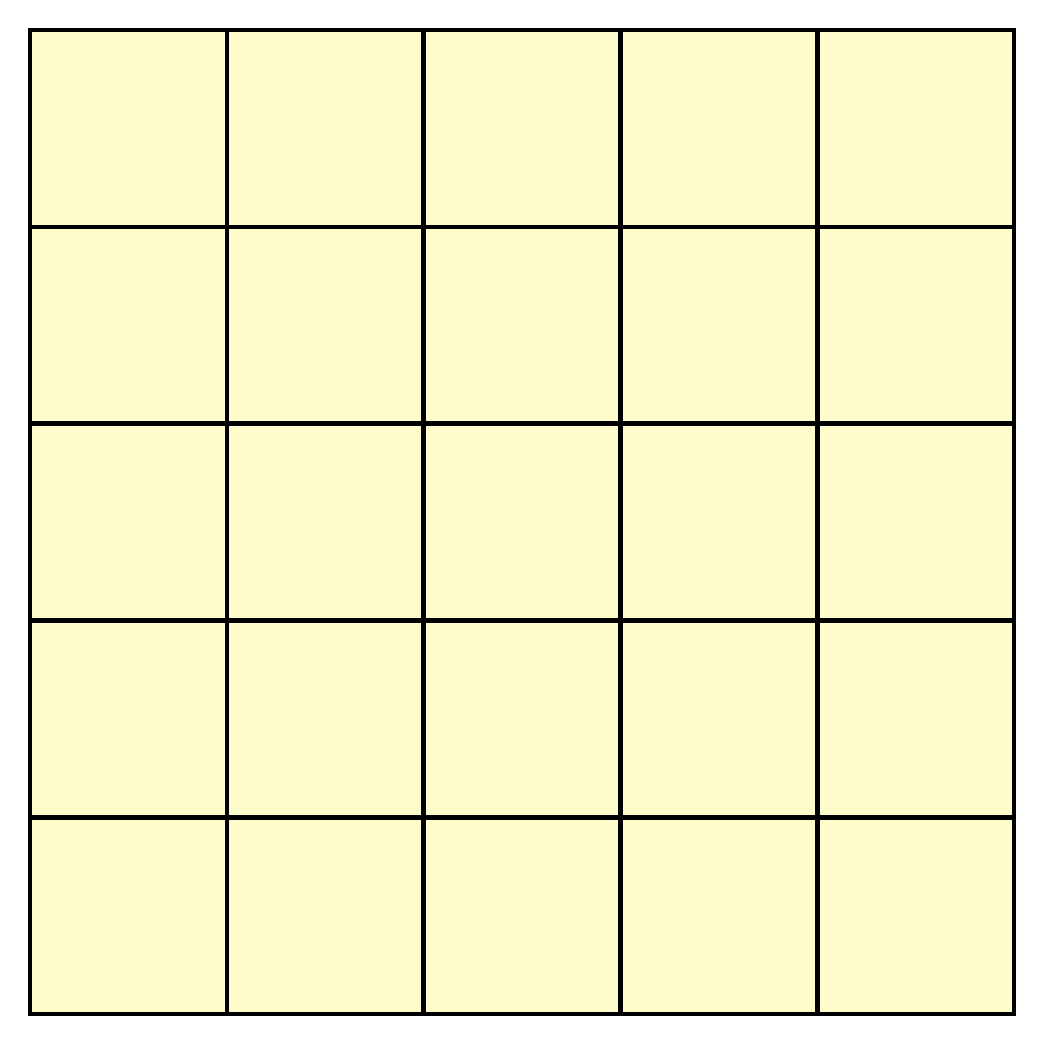
\begin{tikzpicture}[draw=black, ultra thick, x=\Size,y=\Size]
      \foreach \col/\colLetter in \Sequence {%
         \foreach \row/\rowLetter in \Sequence{%
            \pgfmathtruncatemacro{\value}{\col+\NumOfColumns*(\row-1)}
            \def\NodeText{\expandafter\csname Node\rowLetter\colLetter\endcsname}
            \node [Square] at ($(\col,-\row)-(0.5,0.5)$) {\NodeText};
         }
      }
   \end{tikzpicture}
\end{center}
\end{document}
